\documentclass{article}

% Margins
\topmargin=-0.45in
\evensidemargin=0in
\oddsidemargin=0in
\textwidth=6.5in
\textheight=9.0in
\headsep=0.25in

\usepackage{bm,amsmath,subfigure,graphicx,url,algorithm,algorithmicx,algpseudocode,booktabs}
\usepackage{tikz-cd,adjustbox,amsfonts,mathtools,tabularx,capt-of,longtable,comment,caption,soul}
\usepackage[flushleft]{threeparttable}
\usepackage[top=1in,bottom=1in,right=1in,left=1in]{geometry}
\usepackage[backend=bibtex]{biblatex}
\usepackage[titletoc]{appendix}
\usepackage{pgfplots}
\pgfplotsset{compat=1.12}
\usepackage[linktocpage=true]{hyperref}
\usetikzlibrary{shapes.geometric,arrows,automata,positioning}
\usepackage{chngcntr}
\usepackage[final]{pdfpages}
\usepackage[explicit]{titlesec}

\definecolor{lightyellow}{cmyk}{0,0,0.5,0}
\sethlcolor{lightyellow}

\newcommand{\highlight}[1]{%
  \colorbox{yellow!50}{$\displaystyle#1$}}

\newtheorem{theorem}{Theorem}
\newtheorem{corollary}[theorem]{Corollary}
\newtheorem{question}[theorem]{Question}
\newtheorem{lemma}[theorem]{Lemma}
\newtheorem{observation}[theorem]{Observation}
\newtheorem{proposition}{Proposition}
\newtheorem{definition}[theorem]{Definition}
\newtheorem{claim}[theorem]{Claim}
\newtheorem{fact}[theorem]{Fact}
\newtheorem{assumption}[theorem]{Assumption}
\newtheorem{example}{Example}
\newtheorem{conjecture}[theorem]{Conjecture}
\newtheorem{alg}[theorem]{Algorithm}

\newcommand{\set}[1]{{\left\{#1\right\}}}    
\newcommand{\norm}[1]{{||#1||}} 
\newcommand{\abs}[1]{\left\lvert #1 \right\rvert}
\newcommand{\complex}{{\mathbb C}}
\newcommand{\reals}{{\mathbb R}}
\newcommand{\Rho}{\mathrm{P}}
\newcommand{\ints}{{\mathbb Z}}
\newcommand{\nats}{{\mathbb N}}
\newcommand{\proc}{{\mathcal P}}
\newcommand{\enc}[1]{\left<#1\right>}
\newcommand{\tup}[1]{\left(#1\right)}
\newcommand{\code}[1]{\mathtt{#1}}
\newcommand{\spa}[1]{\mathcal{#1}}

\newcommand{\quotes}[1]{``#1''}
\newcommand{\timet}[1]{$t$}
\newcommand{\iitem}{\item[-]}

\usepackage{multicol,calc}

\begin{document}

\tikzstyle{decision} = [diamond, draw, text centered, inner sep=3pt]
\tikzstyle{block} = [rectangle, draw, fill=gray!20,text width=5em, text centered, rounded corners, minimum height=4em]
\tikzstyle{arrow} = [thick,->,>=stealth]

%%%% SVR

\begin{figure}[t!]
\centering
\begin{minipage}{0.65\textwidth}
\small \centering
\[\begin{tikzcd}[column sep = small, row sep = small]
& & \mathcal{D}_1 :  [\bm X][\bm Y_1]  \arrow[rr]  & & h_1 :  \mathcal{D}_1 \rightarrow \bm{\hat{Y_1}}\\
& & \mathcal{D}_2 :  [\bm X][\bm Y_2]  \arrow[rr] & & h_2 :  \mathcal{D}_2 \rightarrow \bm{\hat{Y_2}} \\        
\mathcal{D} :  [\bm X][\bm Y]  \arrow[uurr, bend left=45] \arrow[urr, bend left] \arrow[drr, bend right]  		& & \vdots \\
& & \mathcal{D}_m :  [\bm X][\bm Y_m] \arrow[rr] & & h_m :  \mathcal{D}_m \rightarrow \bm{\hat{Y}_m}
\end{tikzcd}\]
\caption*{\small SVR Flow Diagram. Firstly, the multi-target dataset is divided into $m$ ST datasets, $\mathcal{D}_1, \mathcal{D}_2, \ldots, \mathcal{D}_m$. Then $m$ models, $h_1, h_2, \ldots, h_m$, are independently trained for each ST dataset.}
\end{minipage}
\begin{minipage}{0.65\textwidth}
\begin{algorithm}[H]
\caption*{Multi-Target Support Vector Regression (SVR)} \label{alg:SVR} 
\small \centering
\begin{algorithmic}[1]
\renewcommand{\algorithmicrequire}{\textbf{Input:}}
\renewcommand{\algorithmicensure}{\textbf{Output:}}
\Require Training dataset $\mathcal{D}$
\Ensure  ST models $h_j, j = 1,\ldots,m$
\For {$j = 1$ to $m$}
\State $\mathcal{D}_j = \{\bm X, \bm Y_j\}$ \Comment{Get ST data}
\State $h_j : \bm X \rightarrow \mathbb{R}$ \Comment{Build ST model for the $j^{th}$ target}
\EndFor 
\end{algorithmic} 
\end{algorithm}
\end{minipage}
\end{figure}

%%% BUILD CHAINED MODEL
\begin{figure}[t!]
\centering
\begin{minipage}{0.65\textwidth}
\begin{algorithm}[H]
\centering \small
\caption*{Build Chained Model}
\begin{algorithmic}[1]
\renewcommand{\algorithmicrequire}{\textbf{Input:}}
\renewcommand{\algorithmicensure}{\textbf{Output:}}
\Require Training dataset $\mathcal{D}$, random chain $\bm C$
\Ensure  A chained model $h_j, j = \{1,\ldots,m\}$
\State $\mathcal{D}_1 = \set{\bm X, \bm Y_{\bm C_1}}$ \Comment{Initialize first dataset}
\For {$j=1$ to $m$} \Comment{For each target in chain $\bm C$}
\State $h_j : \mathcal{D}_j \rightarrow \mathbb{R}$ \Comment{Train model on appended dataset}
\If {$j < m$}
\State $\mathcal{D}_{j+1} = \set{\mathcal{D}_j, \bm Y_{\bm C_j}}$ \Comment{Append new target in chain to dataset}
\EndIf
\EndFor 
\end{algorithmic} 
\end{algorithm}
\end{minipage}
\end{figure}


%%% SVRRC 

\begin{figure}[t!]
\centering \small
\begin{minipage}{0.65\textwidth}
\centering \small
\begin{tikzcd}[column sep = small, row sep = small]
& \mathcal{D} :  [\bm X][\bm Y_1 \bm Y_2 \bm Y_3] \arrow[dl] \arrow[d] \arrow[drr] & & \\
\left[1,2,3\right] \arrow[d] & \left[1,3,2\right] \arrow[d] & \hdots & \left[3,2,1\right] \arrow[d] \\
h_1 :  [\bm X] \rightarrow \bm{\hat{Y_1}} \arrow[d] & h_1 :  [\bm X] \rightarrow \bm{\hat{Y_1}} \arrow[d] & \hdots & h_1 :  [\bm X] \rightarrow \bm{\hat{Y_1}} \arrow[d] \\
h_2 :  [\bm X \bm{Y_1} ] \rightarrow \bm{\hat{Y_2}} \arrow[d] & h_2 :  [\bm X \bm{Y_1} ] \rightarrow \bm{\hat{Y_3}} \arrow[d] & \hdots & h_2 :  [\bm X \bm{Y_3} ] \rightarrow \bm{\hat{Y_2}} \arrow[d] \\
h_3 :  [\bm X \bm{Y_1Y_2} ] \rightarrow \bm{\hat{Y_3}} & h_3 :  [\bm X \bm{Y_1Y_3} ] \rightarrow \bm{\hat{Y_2}} & \hdots & h_3 :  [\bm X \bm{Y_3Y_2} ] \rightarrow \bm{\hat{Y_1}}
\end{tikzcd}
\caption*{\small SVRRC Flow Diagram on a dataset with three targets. SVRRC first builds the six random chains of the target's indices (three examples are shown). It then constructs a chained model by proceeding recursively over the chain, building a model, and appending the current target to the input space to predict the next target in the chain. } 
\end{minipage}
\begin{minipage}{0.65\textwidth}
\begin{algorithm}[H]
\caption*{Multi-Target SVR with Random-Chains (SVRRC)}
\small \centering
\label{alg:SVRRC} 
\begin{algorithmic}[1]
\renewcommand{\algorithmicrequire}{\textbf{Input:}}
\renewcommand{\algorithmicensure}{\textbf{Output:}}
\Require Training dataset $\mathcal{D}$, $c$ random chains $\mathcal{C}$
\Ensure  An ensemble of chained models $h_\mathcal{C}$
\For {\textbf{each }$\bm C \in \mathcal{C}$} \Comment{For each random chain}
\State $h_{\bm C} \leftarrow  \mathtt{build Chained Model} (\mathcal{D},\bm C)$ \Comment{Build a chained model for chain $\bm C$}
\EndFor 
\end{algorithmic} 
\end{algorithm}
\end{minipage}
\end{figure}

%%%% SVRCC

\begin{figure}[t!]
\centering \small
\begin{minipage}{0.65\textwidth}
\centering \small
\begin{tikzcd}
\mathcal{D} :  [\bm X][\bm Y_1 \bm Y_2 \bm Y_3] \arrow{rr}{\textit{generate maximum correlation chain}}[swap]{\frac{\mathbf{E}\left[(Y_i - \mu_i)(Y_j - \mu_j)\right]}{\sqrt{\mathbf{E}\left[(Y_i - \mu_i)(Y_i - \mu_i)\right]\mathbf{E}\left[(Y_j - \mu_j)(Y_j - \mu_j)\right]}}} 
&  \arrow[d, phantom, ""{coordinate, name=Z}]
& \left[1,2,3\right]  \arrow[dll, rounded corners, to path={ -- ([xshift=1ex]\tikztostart.east)
|- ([yshift=-2.5ex]Z) [near end]\tikztonodes
-| ([xshift=-1ex]\tikztotarget.west)
-- (\tikztotarget)}] \\
h_1 :  [\bm X] \rightarrow \bm{\hat{Y_1}} \arrow[r]
& h_2 :  [\bm X \bm{Y_1} ] \rightarrow \bm{\hat{Y_2}} \arrow[r]
& h_3 :  [\bm X \bm{Y_1Y_2} ] \rightarrow \bm{\hat{Y_3}} 
\end{tikzcd}
\caption*{\small SVRCC Flow Diagram on a sample dataset with three targets. SVRCC first finds the direction of maximum correlation among the targets and uses that order as the only chain. It then constructs the chained model, as done in SVRRC. } 
\end{minipage}
\begin{minipage}{0.65\textwidth}
\begin{algorithm}[H]
\caption*{Multi-Target SVR with max-Correlation Chain (SVRCC)} 
\centering \small
\begin{algorithmic}[1]
\renewcommand{\algorithmicrequire}{\textbf{Input:}}
\renewcommand{\algorithmicensure}{\textbf{Output:}}
\State $\bm \Rho = corrcoef(\bm Y)$ \Comment{Find correlation coefficient matrix for target variables}
\State $\bm C = \sum_{i=1}^n \bm \Rho_{ij}, \forall j=1,\ldots,m$ \Comment{Sum rows of the correlation matrix}
\State $\bm C = \mathtt{sort}\left(\bm C,\textbf{decreasing}\right)$ \Comment{Sort sums in decreasing order}
\State $h_{\bm C} = \mathtt{buildChainedModel} (\mathcal{D},\bm C)$ \Comment{Build a max-correlation chained model} 
\end{algorithmic} 
\end{algorithm}
\end{minipage}
\end{figure}

\newpage

\begin{table}[t!]
\centering \small
\caption*{Average Relative Root Mean Square Error (aRRMSE) for MT regressors}\vspace{-1em}
\resizebox{0.95\textwidth}{!}{\begin{tabular}{l@{\extracolsep{\fill}}ccccccccccc}
\noalign{\smallskip}\hline\noalign{\smallskip}
Datasets &MORF &ST &MTS &MTSC &RC &ERC &ERCC &SVR &SVRRC &SVRCC \\
\noalign{\smallskip}\hline\noalign{\smallskip}
Slump &0.6939 &0.6886 &0.6690 &0.6938 &0.7019 &0.7022 &0.6886 &0.5765 &\textbf{0.5545} &0.5560   \\
Polymer &0.6159 &0.5971 &0.5778 &0.6493 &0.6270 &0.6544 &0.6131 &0.5573 &0.5253 &\textbf{0.5116}   \\
Andro &0.5097 &0.5979 &0.5155 &0.5633 &0.5924 &0.5885 &0.5666 &0.4856 &0.4651 &\textbf{0.4455}   \\
EDM &0.7337 &0.7442 &0.7413 &0.7446 &0.7449 &0.7452 &0.7443 &0.7058 &0.7070 &\textbf{0.6978}   \\
Solar Flare 1 &1.3046 &1.1357 &1.1168 &1.0758 &0.9951 &1.0457 &1.0887 &0.9917 &0.9455 &\textbf{0.9320}   \\
Jura &0.5969 &0.5874 &0.5906 &0.5892 &0.5910 &0.5896 &0.5880 &0.5952 &\textbf{0.5764} &0.5885   \\
Enb &0.1210 &0.1165 &0.1231 &0.1211 &0.1268 &0.1250 &0.1139 &0.0977 &0.0910 &\textbf{0.0899}   \\
Solar Flare 2 &1.4167 &1.1503 &\textbf{0.9483} &1.0840 &1.0092 &1.0522 &1.0928 &1.0385 &1.0253 &1.0298   \\
Wisconsin Cancer &0.9413 &0.9314 &0.9308 &0.9336 &\textbf{0.9305} &0.9313 &0.9323 &0.9555 &0.9483 &0.9427   \\
California Housing &0.6611 &0.6447 &0.6974 &0.6630 &0.7131 &0.6690 &0.6146 &0.6130 &0.5945 &\textbf{0.5852}   \\
Stock &0.1653 &0.1844 &0.1787 &0.1803 &0.1802 &0.1789 &0.1752 &0.1364 &\textbf{0.1337} &0.1388   \\
SCPF &0.8273 &0.8348 &0.8436 &0.8308 &0.8263 &0.8105 &0.8290 &0.8164 &0.8037 &\textbf{0.8013}   \\
Puma8NH &0.7858 &0.8142 &0.8118 &0.8311 &0.8199 &0.8205 &0.8207 &\textbf{0.7655} &0.7744 &0.7676   \\
Friedman &0.9394 &0.9214 &0.9231 &0.9210 &0.9231 &0.9209 &0.9204 &0.9218 &0.9208 &\textbf{0.9196}   \\
Puma32H &0.9406 &\textbf{0.8713} &0.8727 &0.8791 &0.8752 &0.8729 &0.8740 &0.9364 &0.9367 &0.9319   \\
Water Quality &\textbf{0.8994} &0.9085 &0.9109 &0.9093 &0.9121 &0.9097 &0.9057 &0.9343 &0.9310 &0.9045   \\
M5SPEC &0.5910 &0.5523 &0.5974 &0.5671 &0.5552 &0.5542 &0.5558 &0.2951 &0.2935 &\textbf{0.2925}   \\
MP5SPEC &0.5522 &0.5120 &0.5683 &0.5133 &0.5145 &0.5143 &0.5119 &0.2484 &\textbf{0.2323} &0.2358   \\
MP6SPEC &0.5553 &0.5152 &0.5686 &0.5119 &0.5198 &0.5187 &0.5109 &0.2850 &0.2669 &\textbf{0.2623}   \\
ATP7d &0.5563 &0.5308 &\textbf{0.5141} &0.5142 &0.5558 &0.5397 &0.5182 &0.5455 &0.5371 &0.5342   \\
OES97 &0.5490 &0.5230 &0.5229 &0.5217 &0.5239 &0.5237 &0.5222 &0.4641 &\textbf{0.4618} &0.4635   \\
Osales &0.7596 &0.7471 &\textbf{0.7086} &0.7268 &0.8318 &0.7258 &0.7101 &0.7924 &0.7924 &0.7811   \\
ATP1d &0.4173 &0.3732 &0.3733 &0.3712 &0.3790 &\textbf{0.3696} &0.3721 &0.3773 &0.3707 &0.3775   \\
OES10 &0.4518 &0.4174 &0.4176 &0.4171 &0.4178 &0.4180 &0.4166 &0.3570 &0.3555 &\textbf{0.3538}   \\
\noalign{\smallskip}\hline\noalign{\smallskip}
Average &0.6910 &0.6625 &0.6551 &0.6589 &0.6611 &0.6575 &0.6536 &0.6039 &0.5935 &\textbf{0.5893}   \\
Ranks &7.5000 &5.7708 &5.9375 &6.1667 &7.4375 &6.3750 &4.9792 &4.7708 &3.2708 &\textbf{2.7917}   \\
\noalign{\smallskip}\hline
\end{tabular}}
\end{table}

\begin{table}[t!]
\centering \small
\caption*{Run Time (seconds) for MT regressors}\vspace{-1em}
\resizebox{0.95\textwidth}{!}{\begin{tabular}{l@{\extracolsep{\fill}}rrrrrrrrrrr}
\noalign{\smallskip}\hline\noalign{\smallskip}
Datasets &MORF &ST &MTS &MTSC &RC &ERC &ERCC &SVR &SVRRC &SVRCC \\
\noalign{\smallskip}\hline\noalign{\smallskip}
Slump &38.1 &2.6 &9.9 &15.9 &1.8 &11.1 &50.5 &\textbf{0.6} &1.9 &0.7   \\
Polymer &7.6 &2.7 &9.1 &15.5 &1.9 &14.9 &80.5 &\textbf{0.5} &2.6 &\textbf{0.5}   \\
Andro &25.7 &4.4 &15.0 &34.2 &3.4 &33.2 &197.9 &\textbf{1.1} &6.2 &\textbf{1.1}   \\
EDM &24.8 &2.8 &9.4 &18.1 &2.1 &5.8 &19.0 &\textbf{0.9} &1.0 &\textbf{0.9}   \\
Solar Flare 1 &34.1 &3.5 &13.6 &26.7 &2.7 &17.7 &86.9 &\textbf{2.3} &9.3 &2.6   \\
Jura &64.3 &7.9 &31.8 &74.3 &6.4 &43.5 &254.2 &\textbf{4.7} &18.7 &5.3   \\
Enb &71.4 &6.6 &26.1 &63.6 &\textbf{5.4} &15.6 &69.6 &11.3 &17.7 &15.9   \\
Solar Flare 2 &55.4 &7.4 &30.7 &68.0 &\textbf{6.3} &42.9 &241.5 &9.4 &53.5 &15.6   \\
Wisconsin Cancer &51.4 &6.1 &21.9 &53.7 &4.9 &14.8 &61.6 &\textbf{2.0} &2.4 &\textbf{2.0}   \\
California Housing &93.0 &9.7 &34.8 &75.9 &\textbf{8.2} &21.3 &102.0 &15.8 &25.2 &23.6   \\
Stock &93.7 &11.7 &46.8 &96.7 &\textbf{11.0} &75.4 &427.3 &18.5 &90.5 &26.3   \\
SCPF &66.3 &19.3 &65.9 &176.3 &\textbf{15.0} &104.2 &734.2 &32.8 &162.8 &48.8   \\
Puma8NH &130.4 &29.7 &106.7 &288.6 &\textbf{27.9} &201.6 &1227.7 &94.1 &516.6 &177.1   \\
Friedman &79.5 &27.0 &81.2 &258.3 &25.0 &273.7 &2871.6 &\textbf{12.3} &322.3 &18.8   \\
Puma32H &93.9 &68.1 &181.0 &635.0 &87.7 &667.9 &6087.0 &\textbf{32.2} &1018.7 &53.1   \\
Water Quality &108.4 &\textbf{93.1} &262.1 &912.3 &127.2 &925.4 &10993.3 &110.2 &2567.9 &189.5   \\
M5SPEC &89.8 &68.9 &166.3 &604.6 &73.7 &262.3 &3132.1 &\textbf{39.2} &546.7 &45.1   \\
MP5SPEC &84.5 &94.6 &221.2 &888.3 &91.5 &557.0 &6864.1 &\textbf{49.3} &1132.1 &58.4   \\
MP6SPEC &90.3 &93.4 &212.6 &871.0 &89.1 &557.6 &6761.3 &\textbf{47.2} &1227.1 &58.5   \\
ATP7d &\textbf{70.5} &262.6 &452.1 &2319.8 &242.1 &1779.2 &24373.8 &80.0 &1897.4 &136.5   \\
OES97 &\textbf{83.4} &485.3 &1146.6 &4928.9 &499.8 &5315.0 &58072.1 &148.2 &3759.1 &342.6   \\
Osales &\textbf{92.0} &1094.8 &2340.7 &8322.2 &986.5 &11361.2 &122265.3 &437.0 &4830.1 &843.6   \\
ATP1d &\textbf{70.7} &272.9 &476.5 &2568.9 &261.9 &2138.9 &26768.9 &95.0 &2127.8 &174.4   \\
OES10 &\textbf{90.0} &738.9 &1633.6 &6682.9 &688.5 &7150.8 &83533.1 &229.1 &5419.4 &577.1   \\
\noalign{\smallskip}\hline\noalign{\smallskip}
Average &71.2 &142.2 &316.5 &1250.0 &136.2 &1316.3 &14803.2 &\textbf{61.4} &1073.2 &117.4   \\
Ranks &5.5 &3.71 &6.0 &8.29 &3.0 &7.08 &9.92 &\textbf{1.88} &6.71 &2.92   \\
\noalign{\smallskip}\hline
\end{tabular}}
\end{table}

\newpage

% MIRSVM Primal & Dual
\begin{equation*}
\centering
\begin{aligned}
\min\limits_{\bm w, b,\bm\xi}& {\,\,} \frac{1}{2}||\bm{w}||^2 + C\sum_I \xi_I, & \max\limits_{\bm \alpha}& \sum_I \alpha_I - \frac{1}{2}\sum_I \sum_{K \in I} \alpha_I \alpha_K Y_I Y_K  \spa{K}\left(\bm{x}_{s_I},\bm{x}_{s_K}\right) \\
\text{s.t.}& {\,\,} Y_I(\langle\bm{w},\bm x_{s_I}\rangle + b) \geq 1 - \xi_I,\, \forall I \in \set{1,\ldots,n}, & \text{s.t.}&  \sum_I{\alpha_IY_I} = 0,\, \\
{} & {\,\,} \xi_I \geq 0,\, \forall I \in \set{1,\ldots,n}, & {} & 0 \leq \alpha_I \leq C,\, \forall I \in \set{1,\ldots,n},  \\
{} & s_I = \underset{i \in I}{\text{argmax}} (\langle \bm w,\, \bm x_i \rangle + b),\, \forall I \in \set{1,\ldots,n}. & {} & s_I = \underset{i \in I}{\text{argmax}}(\bm o_I),\, \forall I \in \set{1,\ldots,n}.
\end{aligned}
\end{equation*}

%%% MIRSVM

\begin{figure}[b!]
\centering \small
\begin{minipage}{\textwidth}
\small
\adjustbox{scale=0.9}{
\begin{tikzpicture}[%
    node distance=4cm,
    on grid,
    auto
  ]
\node[block](A) {Initialize $\bm S$ randomly};
\node(B)[block, right of=A, text width=6em] {Train SVM using QP solver over $\bm S$, set $\bm S_{old} = \bm S$};
\draw[arrow] (A) -- (B);
\node(C)[block, right of=B,text width=6.3em] {Find optimal representatives, $\bm S$, for the current hyperplane};
\draw[arrow] (B) -- (C);
\node(D) [decision,right of=C,fill=gray!55,text width=2cm]{while $\bm S$ has not changed, $\bm S \neq \bm S_{old}$};
\draw[arrow] (C) -- (D);
\node(E) [block,right of=D]{return $\bm \alpha,\, b, \bm S$};
\draw[arrow] (D) -- node {yes} (E);
\draw[arrow] (D.north) --+(0,0.1cm) -| (B.north) node[below,pos=0.25] {no} ;
\end{tikzpicture}}
\caption*{\small A summary of the steps performed by MIRSVM. The representatives are first randomly initialized and continuously updated according to the current hyperplane. Upon completion, the model is returned along with the optimal bag-representatives.}
\end{minipage}
\begin{minipage}{\textwidth}
\begin{algorithm}[H]
\caption*{Multi-Instance Representative SVM (MIRSVM)}
\small
\begin{algorithmic}[1]
\renewcommand{\algorithmicrequire}{\textbf{Input:}}
\renewcommand{\algorithmicensure}{\textbf{Output:}}
\Require Training dataset $\mathcal{D}$, SVM Parameters $C$ and $\sigma$
\Ensure  SVM model parameters $\bm \alpha$ and $b$, Bag Representative IDs $\bm S$
\For {$I \in \set{1,\ldots,n}$}
\State $\bm S_I \leftarrow \text{ rand}\left(|\mathcal{B}_I|,1,1\right)$ \Comment{Assign each bag a random instance}
\EndFor
\While {$\bm S \neq \bm S_{old}$}
\State $\bm S_{old} \leftarrow \bm S$
\State $\bm X_S \leftarrow \bm X(\bm S),\,\bm Y_S \leftarrow \bm Y(\bm S)$ \Comment{Initialize the representative dataset}
\State $\bm G \leftarrow (\bm Y_S \times \bm Y_S) \bm \cdot \mathcal{K}\left( \bm X_S,\,\bm X_S,\,\sigma\right)$ \Comment{Build Gram matrix}
\State $\bm \alpha \leftarrow \text{ quadprog}\left(\bm G, \bm{-1}^n, \bm Y_S, \bm 0^n, \bm 0^n, \bm C^n\right)$ \Comment{Solve QP Problem}
\State $\bm{sv} \leftarrow \text{find}\left(0 < \bm \alpha \leq C \right)$ \Comment{Get the support vector indices}
\State $n_{\bm{sv}} \leftarrow \text{count}\left(0 < \bm \alpha \leq C \right)$ \Comment{Get the number of support vectors}
\State $b \leftarrow \frac{1}{n_{\bm{sv}}}\sum_{i=1}^{n_{\bm{sv}}} \left(\bm Y_{\bm{sv}} - \bm G_{\bm{sv}}*\left(\bm{\alpha_{\bm{sv}}} \cdot \bm Y_{\bm{sv}}\right)\right)$ \Comment{Calculate the bias term}
\For {$I \in \set{1,\ldots,n}$} 
\State $\bm G_I \leftarrow (Y_I \times \bm Y_S) \bm \cdot \mathcal{K}\left( \mathcal{B}_I,\,\bm X_S,\,\sigma\right)$
\State $\bm S_I \leftarrow \text{argmax}_{i \in I}\left(\bm G_I*\bm{\alpha} + b \right)$ \Comment{Select optimal bag-representatives}
\EndFor
\EndWhile 
\end{algorithmic}
\end{algorithm}
\end{minipage}
\end{figure}

\begin{figure}[H]
\centering
\begin{minipage}[b]{0.45\textwidth}
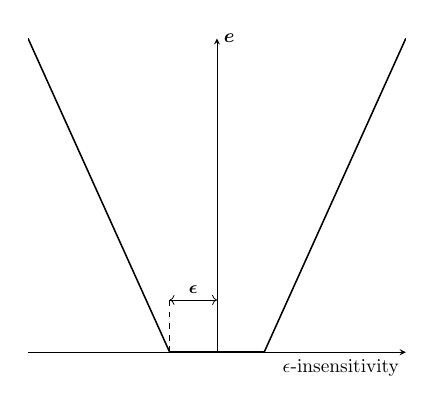
\begin{tikzpicture}[scale=0.7]
\begin{axis}[
	ticks=none,
    axis lines = center, 
    xlabel = $\epsilon\text{-insensitivity}$, 
    xlabel style={below left},
    ylabel = $\bm e$,
    ylabel style={ right}]
% negative epsilon intensity
\addplot [
	thick,
    domain=-4:-1, 
    samples=2, 
    color=black,
]
{- x - 1};
% 0 epsilon intensity
\addplot [
	very thick,
    color=black,
]
coordinates {(-1, 0) (1, 0)};
% positive epsilon intensity
\addplot [
	thick,
    domain=1:4, 
    samples=2, 
    color=black,
]
{ x - 1};
% vertical line indicating where epsilon begines
\addplot[
	color=black,
	style=dashed,
]
coordinates {(-1, 0) (-1, 0.5)};
% epsilon node
\draw[<->] (-1, 0.5) -- (0, 0.5);
\draw (-0.5,0.6) node[font=\small] {$\bm \epsilon$};
\end{axis}
\end{tikzpicture}
\caption{Vapnik's $\epsilon$-insensitivity loss function.}
\label{fig:epsloss}
\end{minipage}
\hfill
\begin{minipage}[b]{0.45\textwidth}
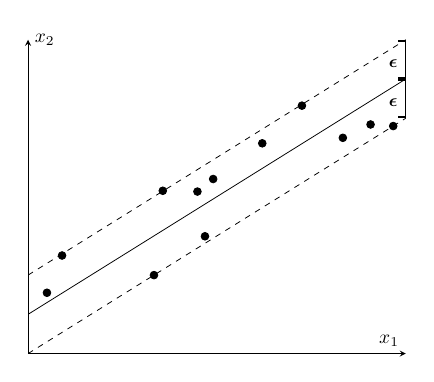
\begin{tikzpicture}[scale = 0.7]
\begin{axis}[
	ticks = none, 
	axis lines = left, 
	xlabel = $x_1$, 
	xlabel style={at={(1,0)}, above left},
	ylabel = $x_2$,
	ylabel style={at={(0,1)}, right,rotate=-90}
    ]
% main function x
\addplot [
    domain=0:6, 
    samples=2, 
    color=black,
]
{x};
% margin function x + eps
\addplot [
	dashed,
    domain=0:6, 
    samples=2, 
    color=black,
]
{ x+1};
% margin function x - eps
\addplot [
	dashed,
    domain=0:6, 
    samples=2, 
    color=black,
]
{ x - 1};
% epsilon margin
\draw[|-|,very thick] (6,7) -- (6,6);
\draw[|-|,very thick] (6,6) -- (6,5);
\draw (5.8,6.4) node[font=\small] {$\bm \epsilon$};
\draw (5.8,5.4) node[font=\small] {$\bm \epsilon$};
\addplot[color=black,only marks, mark size=2] coordinates {(0.54,1.5) (2,1) (2.14,3.15) (2.94,3.45) (5.8,4.8) (0.30,0.55) (2.69,3.13) (2.81,1.99) (3.72,4.36) (4.35,5.32) (5.44,4.84) (5,4.5) };
\end{axis}
\end{tikzpicture}
\caption{Linear support vector regression example solution on a toy 2D dataset.}
\label{fig:regressionsvm}
\end{minipage}
\end{figure}

\newpage

\begin{equation}
\label{eqn:reghingeloss}
\min\limits_{\bm (\bm{w},b) \in \mathcal{H}_o \times \reals} R {\,\,} = {\,\,} \frac{1}{2}||\bm{w}||^2 + C\sum_{i=1}^n L(y_i,\, o_{(w,b)}(\bm{x}_i))
\end{equation}

\begin{equation}\label{eqn:hingeloss}
\centering
L(y_i,\, o_{(w,b)}(\bm{x}_i)) = \max \set{0, 1 - y_i o_{(w,b)}(\bm{x}_i)}
\end{equation}

\begin{equation}
\label{eq:regsvmemp}
\min\limits_{(\bm{w},b) \in \mathcal{H}_o \times \reals} R {\,\,} = {\,\,} \frac{1}{2}||\bm{w}||^2 + C\sum_{i=1}^n (|y_i - o_{(w,b)}(\bm{x_i})|_\epsilon)
\end{equation}

\begin{equation}
\label{eq:epsloss}
\centering
L(y_i,\, o_{(w,b)}(\bm{x}_i)) = \begin{cases} 
															0 & if |y_i - o_{(w,b)}(\bm{x_i})| \leq \epsilon \\
															|y_i - o_{(w,b)}(\bm{x_i})| - \epsilon & \text{otherwise}.
														\end{cases}
\end{equation}

\newpage

\begin{figure}
\centering \small
\begin{minipage}{\textwidth}
\small
\adjustbox{scale=0.9}{
\begin{tikzpicture}[%
    node distance=4cm,
    on grid,
    auto
]
\node[block](A) {Initialize training variables};
\node(B)[block, right of=A, text width=6em] {Calculate updates based on worst-violator and current decision boundary};
\draw[arrow] (A) -- (B);
\node(C)[block, right of=B,text width=6.3em] {Update output vector, worst-violator's alpha, \& bias term};
\draw[arrow] (B) -- (C);
\node(D) [decision,right of=C,fill=gray!55,text width=2cm]{while errors exist};
\draw[arrow] (C) -- (D);
\node(E) [block,right of=D]{return $\bm \alpha,\, b, \bm S$};
\draw[arrow] (D) -- node {no} (E);
\draw[arrow] (D.south) --+(0,-0.7cm) -| (B.south) node[below,pos=0.25] {yes} ;
\end{tikzpicture}}
\caption*{Summary of the steps performed by OLLAWV. The model parameters ($\bm \alpha$, $b$, $\bm S$) and the algorithm variables ($\bm o$, $t$, $wv$, and $yo$) are first initialized. The worst-violator with respect to the current hyperplane is then found and the model parameters are updated. Once no violating samples are found, the model is returned.}
\end{minipage}
\begin{algorithm}[H]
\caption*{OnLine Learning Algorithm using Worst-Violators (OLLAWV)}
\small
\begin{algorithmic}[1]
\renewcommand{\algorithmicrequire}{\textbf{Input:}}
\renewcommand{\algorithmicensure}{\textbf{Output:}}
\Require $\mathcal{D}$, $C$, $\gamma$, $\beta$, $M$
\Ensure  $\bm \alpha$, $b$, $\bm S$
\State $\bm \alpha \leftarrow \bm 0,\, b \leftarrow 0, \bm S \leftarrow \bm 0$ \Comment{Initialize OLLAWV model parameters}
\State $\bm o \leftarrow \bm 0,\, t \leftarrow 0$ \Comment{Initialize the output vector and iteration counter}
\State $wv \leftarrow 0,\, yo \leftarrow y_{wv}*\bm{o}_{wv}$ \Comment{Initialize hinge loss error and worst-violator index}
\While {$yo < M$}
\State $t \leftarrow t + 1$
\State $\eta \leftarrow 2/\sqrt{t}$ \Comment{Learning rate}
\State 
\State $\Lambda \leftarrow \eta*C*y_{wv}$ \Comment{Calculate hinge loss update}
\State $B \leftarrow \left(\Lambda*\beta\right)/n$ \Comment{Calculate bias update}
\State $\bm o \leftarrow \bm o + \Lambda*\mathcal{K}\left(\bm{x}_{\neg \bm S},\, \bm{x}_{wv}, \gamma \right) + B$ \Comment{Update output vector}
\State $\bm \alpha_{wv} \leftarrow \bm \alpha_{wv} + \Lambda$ \Comment{Update worst-violator's alpha value}
\State $b \leftarrow b + B$ \Comment{Update bias term}
\State
\State $\bm S_t \leftarrow wv$ \Comment{Save index of worst-violator}
\State $\left[yo,\, wv\right] \leftarrow \min\limits_{wv \in \set{\neg \bm S}}\set{y_{wv} \cdot o_{wv}}$ \Comment{Find the worst-violator}
\EndWhile 
\end{algorithmic} 
\end{algorithm}
\end{figure}

\begin{table}[t!]
\caption*{Classification Datasets}
\footnotesize \centering
\begin{tabularx}{0.5\textwidth}{l@{\extracolsep{\fill}}rrr}
\hline\noalign{\smallskip}
Dataset & \# Samples & \# Attributes & \# Classes \\
\noalign{\smallskip}\hline\noalign{\smallskip}
\textbf{\textit{small datasets}} & \\
iris & 150 & 4 &  3  \\ 
teach & 151 & 5 &  3  \\ 
wine & 178 & 13 &  3  \\ 
cancer & 198 & 32 &  2  \\ 
sonar & 208 & 60 &  2  \\ 
glass & 214 & 9 &  6  \\ 
vote & 232 & 16 &  2  \\ 
heart & 270 & 13 &  2  \\ 
dermatology & 366 & 33 &  6  \\ 
prokaryotic & 997 & 20 &  3  \\ 
eukaryotic & 2,427 & 20 &  4  \\ 
\textbf{\textit{medium datasets}} & \\
optdigits & 5,620 & 64 &  10  \\ 
satimage & 6,435 & 36 &  6  \\ 
usps & 9,298 & 256 &  10  \\ 
pendigits & 10,992 & 16 &  10  \\ 
reuters & 11,069 & 8,315 &  2  \\ 
letter & 20,000 & 16 &  26  \\ 
\textbf{\textit{large datasets}} & \\
adult & 48,842 & 123 &  2  \\ 
w3a & 49,749 & 300 &  2  \\ 
shuttle & 58,000 & 7 &  7  \\ 
web (w8a) & 64,700 & 300 &  2  \\ 
ijcnn1 & 141,691 & 22 &  2  \\ 
intrusion & 5,209,460 & 127 &  2  \\  
\noalign{\smallskip}\hline
\end{tabularx}
\end{table}

\newpage

\begin{table}[t!]
\centering \small
\caption*{Comparison of OLLAWV vs. NNISDA and MNSVM}\vspace{-1em}
\resizebox{\textwidth}{!}{\begin{tabularx}{1.3\textwidth}{l@{\extracolsep{\fill}}cccrrrccc}
\noalign{\smallskip}\hline\noalign{\smallskip}
\multicolumn{1}{l}{Dataset} & \multicolumn{3}{c}{Accuracy (\%)} & \multicolumn{3}{c}{Run Time (s)} & \multicolumn{3}{c}{Support Vectors (\%)} \\
\cmidrule(lr){2-4}
\cmidrule(lr){5-7}
\cmidrule(lr){8-10} 
 & OLLAWV & NNISDA & MNSVM & OLLAWV & NNISDA & MNSVM & OLLAWV & NNISDA & MNSVM \\
\noalign{\smallskip}\hline\noalign{\smallskip}
\textbf{\textit{small datasets}} & & & & & & & & & \\
iris & \textbf{97.33} & 94.00 & 96.67 & \textbf{0.05} & 0.27 & 3.57 & \textbf{13.50} & 40.20 & 29.80 \\
teach & 52.32 & 52.31 & \textbf{52.95} & \textbf{0.12} & 0.44 & 8.85 & \textbf{69.19} & 99.80 & 87.40 \\
wine & \textbf{98.87} & 96.60 & 96.60 & \textbf{0.28} & 0.43 & 4.84 & \textbf{15.02} & 44.40 & 48.60 \\
cancer & 80.36 & \textbf{81.86} & 81.38 & \textbf{0.49} & 0.85 & 4.46 & \textbf{42.79} & 83.80 & 89.60 \\
sonar & \textbf{92.32} & 89.48 & 87.57 & \textbf{0.59} & 0.98 & 3.03 & \textbf{31.26} & 73.00 & 66.00 \\
glass & \textbf{72.41} & 67.81 & 69.30 & \textbf{0.46} & 1.01 & 11.94 & \textbf{62.84} & 90.80 & 87.60 \\
vote & \textbf{96.54} & 96.11 & 93.99 & \textbf{0.26} & 0.46 & 1.49 & \textbf{13.36} & 33.20 & 34.00 \\
heart & 82.22 & \textbf{83.33} & \textbf{83.33} & \textbf{0.50} & 0.91 & 6.45 & \textbf{37.69} & 73.00 & 82.00 \\
dermatology & 97.82 & \textbf{98.36} & \textbf{98.36} & \textbf{1.62} & 2.47 & 11.68 & \textbf{36.94} & 59.00 & 59.80 \\
prokaryotic & 88.96 & 88.86 & \textbf{88.97} & \textbf{6.09} & 10.64 & 50.86 & \textbf{29.01} & 51.20 & 49.00 \\
eukaryotic & 77.38 & 79.56 & \textbf{81.21} & 61.95 & \textbf{49.16} & 342.76 & \textbf{54.11} & 76.40 & 72.60 \\
\textbf{\textit{medium datasets}} & & & & & & & & & \\
optdigits & 99.11 & 99.29 & \textbf{99.31} & \textbf{411} & 528 & 787 & \textbf{28.64} & 31.60 & 30.60 \\
satimage & 91.66 & \textbf{92.39} & 92.35 & 1,334 & \textbf{687} & 1,094 & \textbf{20.72} & 45.00 & 44.80 \\
usps & 97.49 & 98.05 & \textbf{98.24} & 10,214 & \textbf{5,245} & 7,777 & \textbf{11.22} & 29.40 & 28.00 \\
pendigits & 99.56 & \textbf{99.62} & 99.61 & \textbf{723} & 909 & 1,500 & \textbf{10.27} & 17.60 & 16.60 \\
reuters & 98.03 & \textbf{98.08} & 97.99 & \textbf{954} & 1,368 & 1,657 & \textbf{8.770} & 18.20 & 18.60 \\
letter & 96.99 & 99.11 & \textbf{99.13} & \textbf{5,259} & 12,009 & 26,551 & \textbf{43.56} & 57.60 & 56.60 \\
\textbf{\textit{large datasets}} & & & & & & & & & \\
adult & 84.75 & 85.07 & \textbf{85.13} & \textbf{21,025} & 72,552 & 123,067 & \textbf{34.66} & 56.00 & 56.60 \\
w3a & \textbf{98.86} & 98.82 & 98.82 & \textbf{6,532} & 15,951 & 24,562 & \textbf{3.270} & 14.60 & 12.40 \\
shuttle & 99.77 & 99.83 & \textbf{99.87} & \textbf{2,833} & 7,420 & 45,062 & \textbf{2.010} & 6.00 & 16.40 \\
web & 98.94 & \textbf{99.00} & 99.00 & \textbf{12,067} & 30,583 & 38,040 & \textbf{4.320} & 13.20 & 10.80 \\
ijcnn1 & 98.31 & 99.34 & \textbf{99.41} & \textbf{162,587} & 296,917 & 370,144 & 16.36 & 11.00 & \textbf{7.600} \\
intrusion & \textbf{99.77} & 99.67 & 99.66 & \textbf{2,402,804} & 4,646,810 & 3,772,113 & \textbf{0.780} & 2.000 & 1.700 \\
\noalign{\smallskip}\hline\noalign{\smallskip}
Average & \textbf{91.29} & 91.15 & 91.25 & \textbf{114,209} & 221,350 & 191,861 & \textbf{25.66} & 44.65 & 43.79 \\
Ranks & \textbf{1.739} & 2.022 & 2.239 & \textbf{1.217} & 1.913 & 2.869 & \textbf{1.087} & 2.609 & 2.304 \\
\noalign{\smallskip}\hline\noalign{\smallskip}
\end{tabularx}}
\\ \vspace{1em}
\begin{minipage}{0.3\textwidth}
\centering
\resizebox{0.9\textwidth}{!}{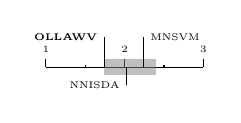
\begin{tikzpicture}
\draw (1,0) -- (3,0);
\foreach \x in {1,2,3} {
\draw (\x, 0) -- ++(0,.1) node [above,scale=0.7] {\tiny \x};
\ifthenelse{\x < 3}{\draw (\x+.5, 0) -- ++(0,.03);}{}
}

\coordinate (c0) at (1.7391,0);
\coordinate (c1) at (2.0217,0);
\coordinate (c2) at (2.2391,0);

\node (l0) at (c0) [above left=.25cm and 0cm, align=right,scale=0.7] {\tiny \textbf{OLLAWV}};
\node (l1) at (c1) [below left=.1cm and 0cm, align=right,scale=0.7] {\tiny NNISDA};
\node (l2) at (c2) [above right=.25cm and 0cm, align=right,scale=0.7] {\tiny MNSVM};

\fill[fill=gray,fill opacity=0.5] (1.7391,-0.1) rectangle (2.3991,0.1);

\foreach \x in {0,1,2} {
\draw (l\x) -| (c\x);
};
\end{tikzpicture}}
\captionsetup{width=0.7\linewidth}
\captionof*{figure}{\small Bonferroni-Dunn test for Accuracy}\label{fig:BonfDunnaccolla}
\end{minipage}
\hspace{0.5em}
\begin{minipage}{0.3\textwidth}
\centering
\resizebox{0.8\textwidth}{!}{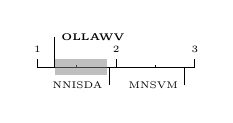
\begin{tikzpicture}
\draw (1,0) -- (3,0);
\foreach \x in {1,2,3}{
\draw (\x, 0) -- ++(0,.1) node [above,scale=0.7] {\tiny \x};
\ifthenelse{\x < 3}{\draw (\x+.5, 0) -- ++(0,.03);}{}
}

\coordinate (c0) at (1.2174,0);
\coordinate (c1) at (1.913,0);
\coordinate (c2) at (2.8696,0);

\node (l0) at (c0) [above right=.25cm and 0cm, align=right,scale=0.7] {\tiny \textbf{OLLAWV}};
\node (l1) at (c1) [below left=.1cm and 0cm, align=right,scale=0.7] {\tiny NNISDA};
\node (l2) at (c2) [below left=.1cm and 0cm, align=right,scale=0.7] {\tiny MNSVM};

\fill[fill=gray,fill opacity=0.5] (1.2174,-0.1) rectangle (1.8774,0.1);

\foreach \x in {0,1,2} {
\draw (l\x) -| (c\x);
};
\end{tikzpicture}}
\captionsetup{width=0.7\linewidth}
\captionof*{figure}{\small Bonferroni-Dunn test for Run Time}\label{fig:BonfDunncpu}
\end{minipage}
\hspace{0.5em}
\begin{minipage}{0.3\textwidth}
\centering
\resizebox{0.8\textwidth}{!}{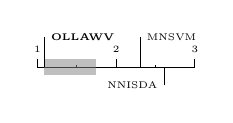
\begin{tikzpicture}
\draw (1,0) -- (3,0);
\foreach \x in {1,2,3} {
\draw (\x, 0) -- ++(0,.1) node [above,scale=0.7] {\tiny \x};
\ifthenelse{\x < 3}{\draw (\x+.5, 0) -- ++(0,.03);}{}
}

\coordinate (c0) at (1.087,0);
\coordinate (c1) at (2.6087,0);
\coordinate (c2) at (2.3043,0);

\node (l0) at (c0) [above right=.25cm and 0cm, align=right,scale=0.7] {\tiny \textbf{OLLAWV}};
\node (l1) at (c1) [below left=.1cm and 0cm, align=right,scale=0.7] {\tiny NNISDA};
\node (l2) at (c2) [above right=.25cm and 0cm, align=right,scale=0.7] {\tiny MNSVM};

\fill[fill=gray,fill opacity=0.5] (1.087,-0.1) rectangle (1.747,0.1);

\foreach \x in {0,1,2} {
\draw (l\x) -| (c\x);
};
\end{tikzpicture}}
\captionsetup{width=0.7\linewidth}
\captionof*{figure}{\small Bonferroni-Dunn test for \% Support Vectors}\label{fig:BonfDunnsv}
\end{minipage}
\end{table}

\newpage

\begin{figure}
\centering
\begin{minipage}{0.3\textwidth}
\centering \small
\resizebox{0.8\textwidth}{!}{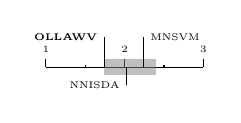
\begin{tikzpicture}
\draw (1,0) -- (3,0);
\foreach \x in {1,2,3} {
\draw (\x, 0) -- ++(0,.1) node [above,scale=0.7] {\tiny \x};
\ifthenelse{\x < 3}{\draw (\x+.5, 0) -- ++(0,.03);}{}
}

\coordinate (c0) at (1.7391,0);
\coordinate (c1) at (2.0217,0);
\coordinate (c2) at (2.2391,0);

\node (l0) at (c0) [above left=.25cm and 0cm, align=right,scale=0.7] {\tiny \textbf{OLLAWV}};
\node (l1) at (c1) [below left=.1cm and 0cm, align=right,scale=0.7] {\tiny NNISDA};
\node (l2) at (c2) [above right=.25cm and 0cm, align=right,scale=0.7] {\tiny MNSVM};

\fill[fill=gray,fill opacity=0.5] (1.7391,-0.1) rectangle (2.3991,0.1);

\foreach \x in {0,1,2} {
\draw (l\x) -| (c\x);
};
\end{tikzpicture}}
\vspace{-0.5em}
\captionsetup{width=0.7\linewidth}
\captionof*{figure}{\small Bonferroni-Dunn test for Accuracy}
\end{minipage}

\vspace{2em}

\begin{minipage}{0.3\textwidth}
\centering \small
\resizebox{0.8\textwidth}{!}{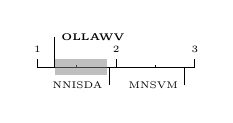
\begin{tikzpicture}
\draw (1,0) -- (3,0);
\foreach \x in {1,2,3}{
\draw (\x, 0) -- ++(0,.1) node [above,scale=0.7] {\tiny \x};
\ifthenelse{\x < 3}{\draw (\x+.5, 0) -- ++(0,.03);}{}
}

\coordinate (c0) at (1.2174,0);
\coordinate (c1) at (1.913,0);
\coordinate (c2) at (2.8696,0);

\node (l0) at (c0) [above right=.25cm and 0cm, align=right,scale=0.7] {\tiny \textbf{OLLAWV}};
\node (l1) at (c1) [below left=.1cm and 0cm, align=right,scale=0.7] {\tiny NNISDA};
\node (l2) at (c2) [below left=.1cm and 0cm, align=right,scale=0.7] {\tiny MNSVM};

\fill[fill=gray,fill opacity=0.5] (1.2174,-0.1) rectangle (1.8774,0.1);

\foreach \x in {0,1,2} {
\draw (l\x) -| (c\x);
};
\end{tikzpicture}}
\vspace{-0.5em}
\captionsetup{width=0.7\linewidth}
\captionof*{figure}{\small Bonferroni-Dunn test for Run Time}
\end{minipage}

\vspace{2em}

\begin{minipage}{0.3\textwidth}
\centering \small
\resizebox{0.8\textwidth}{!}{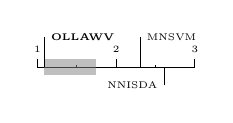
\begin{tikzpicture}
\draw (1,0) -- (3,0);
\foreach \x in {1,2,3} {
\draw (\x, 0) -- ++(0,.1) node [above,scale=0.7] {\tiny \x};
\ifthenelse{\x < 3}{\draw (\x+.5, 0) -- ++(0,.03);}{}
}

\coordinate (c0) at (1.087,0);
\coordinate (c1) at (2.6087,0);
\coordinate (c2) at (2.3043,0);

\node (l0) at (c0) [above right=.25cm and 0cm, align=right,scale=0.7] {\tiny \textbf{OLLAWV}};
\node (l1) at (c1) [below left=.1cm and 0cm, align=right,scale=0.7] {\tiny NNISDA};
\node (l2) at (c2) [above right=.25cm and 0cm, align=right,scale=0.7] {\tiny MNSVM};

\fill[fill=gray,fill opacity=0.5] (1.087,-0.1) rectangle (1.747,0.1);

\foreach \x in {0,1,2} {
\draw (l\x) -| (c\x);
};
\end{tikzpicture}}
\vspace{-0.5em}
\captionsetup{width=0.7\linewidth}
\captionof*{figure}{\small Bonferroni-Dunn test for \% Support Vectors}
\end{minipage}
\end{figure}

\newpage

\begin{table}[b!]
\centering \small
\begin{tabularx}{0.3\textwidth}{c@{\extracolsep{\fill}}}
\begin{minipage}{0.3\textwidth}
\centering \small
\resizebox{0.8\textwidth}{!}{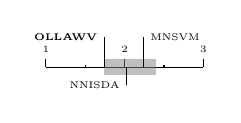
\begin{tikzpicture}
\draw (1,0) -- (3,0);
\foreach \x in {1,2,3} {
\draw (\x, 0) -- ++(0,.1) node [above,scale=0.7] {\tiny \x};
\ifthenelse{\x < 3}{\draw (\x+.5, 0) -- ++(0,.03);}{}
}

\coordinate (c0) at (1.7391,0);
\coordinate (c1) at (2.0217,0);
\coordinate (c2) at (2.2391,0);

\node (l0) at (c0) [above left=.25cm and 0cm, align=right,scale=0.7] {\tiny \textbf{OLLAWV}};
\node (l1) at (c1) [below left=.1cm and 0cm, align=right,scale=0.7] {\tiny NNISDA};
\node (l2) at (c2) [above right=.25cm and 0cm, align=right,scale=0.7] {\tiny MNSVM};

\fill[fill=gray,fill opacity=0.5] (1.7391,-0.1) rectangle (2.3991,0.1);

\foreach \x in {0,1,2} {
\draw (l\x) -| (c\x);
};
\end{tikzpicture}}
\captionsetup{width=0.7\linewidth}
\captionof*{figure}{\small Accuracy (\%)}
\end{minipage}\vspace{1em} \\

\begin{minipage}{0.3\textwidth}
\centering \small
\resizebox{0.8\textwidth}{!}{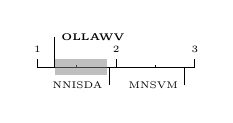
\begin{tikzpicture}
\draw (1,0) -- (3,0);
\foreach \x in {1,2,3}{
\draw (\x, 0) -- ++(0,.1) node [above,scale=0.7] {\tiny \x};
\ifthenelse{\x < 3}{\draw (\x+.5, 0) -- ++(0,.03);}{}
}

\coordinate (c0) at (1.2174,0);
\coordinate (c1) at (1.913,0);
\coordinate (c2) at (2.8696,0);

\node (l0) at (c0) [above right=.25cm and 0cm, align=right,scale=0.7] {\tiny \textbf{OLLAWV}};
\node (l1) at (c1) [below left=.1cm and 0cm, align=right,scale=0.7] {\tiny NNISDA};
\node (l2) at (c2) [below left=.1cm and 0cm, align=right,scale=0.7] {\tiny MNSVM};

\fill[fill=gray,fill opacity=0.5] (1.2174,-0.1) rectangle (1.8774,0.1);

\foreach \x in {0,1,2} {
\draw (l\x) -| (c\x);
};
\end{tikzpicture}}
\captionsetup{width=0.7\linewidth}
\captionof*{figure}{\small Run Time (s)}
\end{minipage}\vspace{1em} \\ 

\begin{minipage}{0.3\textwidth}
\centering \small
\resizebox{0.8\textwidth}{!}{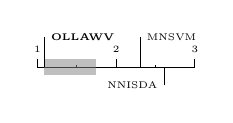
\begin{tikzpicture}
\draw (1,0) -- (3,0);
\foreach \x in {1,2,3} {
\draw (\x, 0) -- ++(0,.1) node [above,scale=0.7] {\tiny \x};
\ifthenelse{\x < 3}{\draw (\x+.5, 0) -- ++(0,.03);}{}
}

\coordinate (c0) at (1.087,0);
\coordinate (c1) at (2.6087,0);
\coordinate (c2) at (2.3043,0);

\node (l0) at (c0) [above right=.25cm and 0cm, align=right,scale=0.7] {\tiny \textbf{OLLAWV}};
\node (l1) at (c1) [below left=.1cm and 0cm, align=right,scale=0.7] {\tiny NNISDA};
\node (l2) at (c2) [above right=.25cm and 0cm, align=right,scale=0.7] {\tiny MNSVM};

\fill[fill=gray,fill opacity=0.5] (1.087,-0.1) rectangle (1.747,0.1);

\foreach \x in {0,1,2} {
\draw (l\x) -| (c\x);
};
\end{tikzpicture}}\\
\captionsetup{width=0.7\linewidth}
\captionof*{figure}{\small Support Vectors (\%)}
\end{minipage} \\
\end{tabularx}
\end{table}

\newpage

\begin{figure}[t!]
\begin{minipage}{0.8\textwidth}
\caption*{Accuracy (\%) for Non-SVM Methods vs. OLLAWV}\vspace{-1em}
\small \centering
\resizebox{\textwidth}{!}{\begin{tabular}{l@{\extracolsep{\fill}}cccccc}
\noalign{\smallskip}\hline\noalign{\smallskip}
Dataset & OLLAWV & $k$-NN & J48 & JRip & Na\"ive Bayes & Logistic \\
\noalign{\smallskip}\hline\noalign{\smallskip}
\textbf{\textit{small datasets}} & & & & & & \\
iris & \textbf{97.33 $\pm$ 1.49} & 96.00 $\pm$ 3.65 & 94.00 $\pm$ 2.79 & 90.67 $\pm$ 4.35 & 96.00 $\pm$ 2.79 & 97.33 $\pm$ 2.79  \\
teach & 52.32 $\pm$ 3.46 & \textbf{59.64 $\pm$ 2.89} & 49.72 $\pm$ 7.58 & 56.75 $\pm$ 9.60 & 53.75 $\pm$ 6.46 & 51.77 $\pm$ 6.68 \\
wine & \textbf{98.87 $\pm$ 1.54} & 97.73 $\pm$ 3.72 & 90.43 $\pm$ 5.83 & 93.24 $\pm$ 3.27 & 96.60 $\pm$ 3.14 & 96.05 $\pm$ 2.58 \\
cancer & \textbf{80.36 $\pm$ 5.80} & 77.32 $\pm$ 6.93 & 73.81 $\pm$ 8.57 & 73.78 $\pm$ 5.81 & 67.73 $\pm$ 5.07 & 77.32 $\pm$ 7.78 \\
sonar & \textbf{92.32 $\pm$ 3.11} & 88.99 $\pm$ 4.59 & 76.16 $\pm$ 10.6 & 75.18 $\pm$ 6.77 & 73.69 $\pm$ 7.65 & 75.18 $\pm$ 7.31 \\
glass & \textbf{72.41 $\pm$ 2.28} & 67.73 $\pm$ 5.91 & 65.06 $\pm$ 5.51 & 65.59 $\pm$ 9.66 & 49.46 $\pm$ 5.19 & 62.04 $\pm$ 5.75 \\
vote & \textbf{96.54 $\pm$ 1.87} & 92.26 $\pm$ 3.19 & 95.70 $\pm$ 2.12 & 96.54 $\pm$ 2.45 & 92.24 $\pm$ 3.24 & 93.54 $\pm$ 2.59 \\
heart & 82.22 $\pm$ 2.93 & 79.63 $\pm$ 5.71 & 78.52 $\pm$ 2.81 & 80.74 $\pm$ 4.06 & \textbf{84.44 $\pm$ 4.46} & 83.33 $\pm$ 3.93 \\
dermatology & \textbf{97.82 $\pm$ 0.05} & 96.18 $\pm$ 1.78 & 94.52 $\pm$ 2.21 & 91.27 $\pm$ 5.08 & 97.28 $\pm$ 1.64 & 96.98 $\pm$ 2.28 \\
prokaryotic & \textbf{88.96 $\pm$ 2.14} & 87.96 $\pm$ 3.01 & 78.54 $\pm$ 1.62 & 79.13 $\pm$ 2.78 & 62.38 $\pm$ 3.54 & 87.57 $\pm$ 2.56 \\
eukaryotic & 77.38 $\pm$ 1.96 & \textbf{81.42 $\pm$ 2.06} & 65.27 $\pm$ 2.92 & 66.42 $\pm$ 3.47 & 39.27 $\pm$ 3.43 & 69.55 $\pm$ 1.34 \\
\textbf{\textit{medium datasets}} & & & & & & \\
optdigits & \textbf{99.11 $\pm$ 0.38} & 98.74 $\pm$ 0.39 & 90.87 $\pm$ 1.09 & 91.28 $\pm$ 0.40 & 92.42 $\pm$ 0.75 & 95.05 $\pm$ 0.91 \\
satimage & \textbf{91.66 $\pm$ 0.80} & 90.38 $\pm$ 0.72 & 85.64 $\pm$ 1.21 & 85.33 $\pm$ 0.77 & 85.41 $\pm$ 0.92 & 88.14 $\pm$ 1.11 \\
usps & \textbf{97.49 $\pm$ 0.22} & 97.04 $\pm$ 0.47 & 88.73 $\pm$ 0.46 & 89.20 $\pm$ 1.00 & 79.45 $\pm$ 0.59 & 91.88 $\pm$ 0.65 \\
pendigits & \textbf{99.56 $\pm$ 0.12} & 99.33 $\pm$ 0.17 & 96.24 $\pm$ 0.31 & 96.34 $\pm$ 0.41 & 88.34 $\pm$ 0.65 & 95.59 $\pm$ 0.18 \\
reuters & \textbf{98.03 $\pm$ 0.22} & 97.15 $\pm$ 0.43 & 96.90 $\pm$ 0.32 & 97.18 $\pm$ 0.44 & 93.52 $\pm$ 0.02 & 69.54 $\pm$ 0.28 \\
letter & \textbf{96.99 $\pm$ 0.21} & 95.71 $\pm$ 0.19 & 87.34 $\pm$ 0.68 & 87.02 $\pm$ 0.66 & 74.12 $\pm$ 0.97 & 77.45 $\pm$ 0.16 \\
\textbf{\textit{large datasets}} & & & & & & \\
adult & \textbf{84.75 $\pm$ 0.26} & 83.85 $\pm$ 0.28 & 84.38 $\pm$ 0.28 & 83.73 $\pm$ 0.17 & 80.57 $\pm$ 0.09 & 82.46 $\pm$ 0.14 \\
w3a & \textbf{98.86 $\pm$ 0.04} & 98.60 $\pm$ 0.06 & 98.71 $\pm$ 0.05 & 98.41 $\pm$ 0.10 & 96.71 $\pm$ 0.20 & 98.61 $\pm$ 0.12 \\
shuttle & 99.77 $\pm$ 0.03 & 99.93 $\pm$ 0.03 & \textbf{99.97 $\pm$ 0.02} & 99.96 $\pm$ 0.02 & 98.57 $\pm$ 0.24 & 96.83 $\pm$ 0.12 \\
web & \textbf{98.94 $\pm$ 0.05} & 98.89 $\pm$ 0.06 & 98.79 $\pm$ 0.09 & 98.50 $\pm$ 0.13 & 96.71 $\pm$ 0.21 & 98.70 $\pm$ 0.08 \\
ijcnn1 & 98.31 $\pm$ 0.07 & \textbf{98.48 $\pm$ 0.04} & 98.40 $\pm$ 0.09 & 98.11 $\pm$ 0.10 & 90.69 $\pm$ 0.26 & 92.29 $\pm$ 0.16 \\
intrusion & \textbf{99.77 $\pm$ 0.02} & 88.20 $\pm$ 1.06 & 58.01 $\pm$ 26.6 & 87.66 $\pm$ 3.79 & 49.75 $\pm$ 30.7 & 65.15 $\pm$ 15.7 \\
\noalign{\smallskip}\hline\noalign{\smallskip}
Average & \textbf{91.29 $\pm$ 1.26} & 90.05 $\pm$ 2.06 & 84.60 $\pm$ 3.64 & 86.18 $\pm$ 2.84 & 79.96 $\pm$ 3.58 & 84.45 $\pm$ 2.83 \\
Ranks & \textbf{1.500} & $2.500$ & $4.041$ & $3.958$ & $5.063$ & $3.938$ \\
\noalign{\smallskip}\hline\noalign{\smallskip}
\end{tabular}}
\end{minipage}
\hspace{1em}
\begin{minipage}{0.13\textwidth}
\centering
\resizebox{\textwidth}{!}{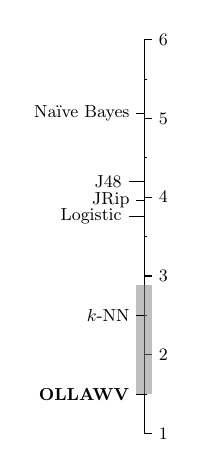
\begin{tikzpicture}
\draw (0,1) -- (0,6);
\foreach \x in {1,2,3,4,5,6} {
\draw (0, \x) -- ++(0.1,0) node [right,scale=0.7] {\small \x};
\ifthenelse{\x < 6}{\draw (0, \x+.5) -- ++(.03, 0);}{}
}

\coordinate (c0) at (0,1.5);
\coordinate (c1) at (0,2.5);
\coordinate (c2) at (0,4.041);
\coordinate (c3) at (0,3.9583);
\coordinate (c4) at (0,5.0625);
\coordinate (c5) at (0,3.9375);

\node (l0) at (c0) [left=0cm and 0.1cm, align=right,scale=0.7] {\small \textbf{OLLAWV}};
\node (l1) at (c1) [left=0cm and 0.1cm, align=right,scale=0.7] {\small $k$-NN};
\node (l2) at (c2) [above left=0cm and 0.2cm, align=right,scale=0.7] {\small J$48$};
\node (l3) at (c3) [left=0cm and 0.1cm, align=right,scale=0.7] {\small JRip};
\node (l4) at (c4) [left=0cm and 0.1cm, align=left,scale=0.7] {\small Na\"{i}ve Bayes};
\node (l5) at (c5) [below left=0cm and 0.2cm, align=right,scale=0.7] {\small Logistic};


\fill[fill=gray,fill opacity=0.5] (-0.1,1.5) rectangle (0.1,2.89);

\foreach \x in {0,1,2,3,4,5} {
\draw (l\x) -| (c\x);
};
\end{tikzpicture}}
\end{minipage}
\end{figure}



\end{document}